\chapter{Affine toric varieties}

\section{Introduction}

\begin{definition}[Affine toric variety]
An \textbf{affine toric variety} is an irreducible affine variety $X$ equipped with an open embedding of a torus $T$ such that the translation action $T\times T\to T$ extends to an action of $T$ on $X$.
\end{definition}

\begin{remark}
The open torus is automatically dense in, and of the same dimension of, $X$.
\end{remark}

\begin{remark}
The extension of the action is unique because if $X$ and $Y$ are irreducible affine and $f,g:X\to Y$ agree on a dense open subset then $f=g$.
\end{remark}

\begin{example}
A torus is a toric variety.
\end{example}

\begin{example}
Affine space $\A^n$ is a toric variety, via the trivial embedding 
\[\G_m^n=\cpa{x_1\cdots x_n\neq 0}\subseteq \A^n.\]
\end{example}

\begin{example}
Let $C=V(x^3-y^2)\subseteq \A^2$ with torus
\[\funcDef{\G_m}{C}{t}{(t^2,t^3)}\]
and action
\[\funcDef{\G_m\times C}{C}{(t,(x,y))}{(t^2x,t^3y)}.\]
Notice that this affine toric variety is neither smooth nor normal\footnote{$\Spec A$ irreducible affine variety is \textbf{normal} if all local rings are integrally closed in $\Frac A$. This is equivalent to $A$ being integrally closed in $\Frac A$.}.
\end{example}

\begin{fact}
A normal variety is smooth in codimension 1, that it, the singular locus has codimension at least 2. In particular a curve is normal iff they're smooth.
\end{fact}


\begin{example}
Let $X=V(xy-z^2)\subseteq \A^3$ be the \textit{quadric cone}. It can be shown that $X$ is normal, but it is not smooth (not at the origin).

\begin{figure}[!htb]
    \centering
    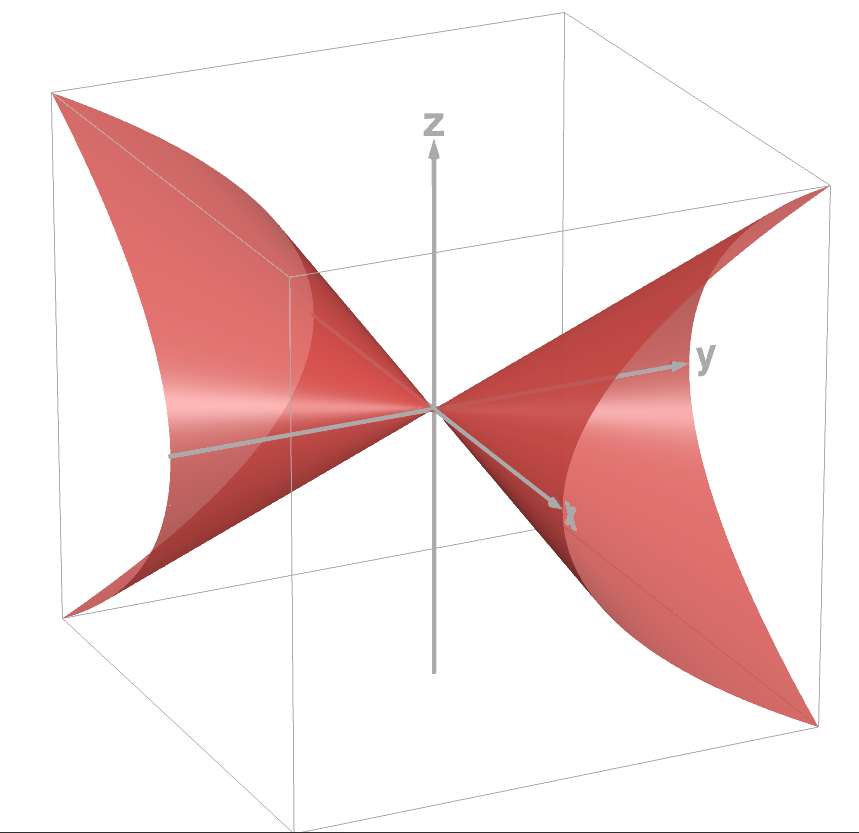
\includegraphics[width=6cm]{Images/quadric cone.png}
    \caption{Quadric cone over the real numbers.}
\end{figure}


$X$ is a toric variety with torus given by the image of\footnote{this map is 2:1, to get the actual parametrization we need
\[\funcDef{\G_m^2}{X}{(s,t)}{(s,st^2,st)}\]
This is related to the fact that $X$ is the quotient $\A^2/\mu_2$ by the action $-1(x,y)=(-x,-y)$.}
\[\funcDef{\G_m^2}{X}{(s,t)}{(s^2,t^2,st)}\]
and action
\[\funcDef{\G_m^2\times X}{X}{((s,t),(x,y,z))}{(sx,st^2y,stz)}\]
\end{example}


\begin{example}
$X=V(xy-zw)\subseteq \A^4$ is a toric variety with torus
\[\funcDef{\G_m^3}{X}{(t_1,t_2,t_3)}{(t_1,t_2,t_3,t_1t_2t_3\ii)}\]
and action 
\[\funcDef{\G_m^3\times X}{X}{((t_1,t_2,t_3),(x,y,z,w))}{(t_1x,t_2y,t_3z,t_1t_2t_3\ii w)}\]
\end{example}


\section{Monoids}

\begin{definition}[Monoid]
A \textbf{monoid} is a set $S$ with an operation $+$, which is commutative, associative and with a neutral element $0\in S$.
\end{definition}

\begin{remark}
The reference book \cite{cox2011toric} calls these \textit{semigroups}.
\end{remark}


\begin{definition}
If $A\subseteq S$ is a subset of a monoid, the \textbf{submonoid generated by $A$ in $S$} is the smallest submonoid which contains $A$. Concretely it is 
\[\ps A=\cpa{\sum_{a\in A} n_a a\mid n_a\in \N,\ n_a=0\text{ for all but finitely many coeff.}}\]
A monoid $S$ is \textbf{finitely generated} if there exists a finite subset $A\subseteq S$ such that $S=\ps A$.
\end{definition}

\begin{remark}
$S$ is a finitely generated monoid if there exists a surjective monoid homomorphism
\[\N^n\onto S.\]
\end{remark}

\begin{definition}
$S$ is an \textbf{affine monoid} if it is finitely generated and it is a submonoid of a lattice $M$.
\end{definition}

\begin{example}
$\N^k\subseteq \Z^k$ is an affine monoid.
\end{example}

\begin{example}
$\znz n$ is a monoid but it is NOT affine because a lattice can't have a submonoid with torsion.
\end{example}

\begin{example}
$\ps{(1,0),(1,1)}\subseteq \N\oplus \znz{2}$ is also not affine because of torsion.
\end{example}

\begin{definition}[Integrality]
A monoid $S$ is \textbf{integral} (or \textbf{cancellative}) if $a+b=a+c\implies b=c$.
\end{definition}

\begin{fact}
A monoid $S$ is affine if and only if $S$ is
\begin{itemize}
\item finitely generated,
\item integral and
\item torsion free.
\end{itemize}
\end{fact}

Let us now define the left adjoint to the forgetful $\Ab\to \Mon$:

\begin{definition}[Associated group]
Let $S$ be a monoid. There is an \textbf{associated abelian group} $S^{gp}$, which is the initial group with a morphism from $S$. Concretely
\[S^{gp}=\frac{\cpa{(s,s')\mid s,s'\in S}}\sim\]
where $(s_1,s'_1)\sim(s_2,s'_2)$ if there exists $s\in S$ such that\footnote{think about localization on rings which are not domains.}
\[s+s_1+s_2'=s+s_2+s_1'.\]
\end{definition}

\begin{remark}
$S^{gp}$ is an abelian group and we have a map $S\to S^{gp}$ given by $s\mapsto [(s,0)]_\sim$.
\end{remark}


\begin{fact}
Any morphism $S\to G$ for $G$ abelian group factors uniquely through $S^{gp}$. More precisely
\[\Hom_{\text{Mon}}(S,G)=\Hom_{\text{Ab}}(S^{gp},G)\]
\end{fact}


\begin{remark}
$S$ is integral if and only if $S\to S^{gp}$ is injective, which happens if and only if $S$ can be injected into an abelian group.
\end{remark}

\subsubsection{Presentations of monoids}
With monoids, the kernel is ``sort of useless"
\begin{example}
Consider
\[\funcDef{\N^2}{\N}{(a,b)}{a+b}\]
this has trivial kernel (preimage of $0$ is just $(0,0)$) but it is far from being injective.
\end{example}

Let $f:S\to S'$ be a surjective homomorphism. What we should look at instead of the kernel for the right analogue of the first isomorphism theorem is
\[E=\cpa{(s,s')\in S\times S\mid f(s)=f(s')}.\]
This set is an equivalence relation on $S\times S$, which is also a submonoid.

\begin{definition}[Congruence relations]
A submonoid of $S\times S$ which defines an equivalence relation is called \textbf{congruence relation}.
\end{definition}

\begin{definition}[Coequalizer]
If $f,g:X\to Y$, the coequalizer is an object $Z$ together with $h:Y\to Z$ such that $h\circ f=h\circ g:X\to Z$ and if $W$ together with $h':Y\to W$ is also such that $h'\circ f=c'\circ g$ then there exists a unique $Z\to W$ making everything commute.
% https://q.uiver.app/#q=WzAsNCxbMCwxLCJYIl0sWzEsMSwiWSJdLFsyLDEsIloiXSxbMiwwLCJXIl0sWzAsMSwiZiIsMCx7Im9mZnNldCI6LTF9XSxbMCwxLCJnIiwyLHsib2Zmc2V0IjoxfV0sWzEsMiwiaCIsMl0sWzEsMywiaCciXSxbMiwzLCJcXGV4aXN0cyEiLDIseyJzdHlsZSI6eyJib2R5Ijp7Im5hbWUiOiJkYXNoZWQifX19XV0=
\[\begin{tikzcd}
	&& W \\
	X & Y & Z
	\arrow["f", shift left, from=2-1, to=2-2]
	\arrow["g"', shift right, from=2-1, to=2-2]
	\arrow["{h'}", from=2-2, to=1-3]
	\arrow["h"', from=2-2, to=2-3]
	\arrow["{\exists!}"', dashed, from=2-3, to=1-3]
\end{tikzcd}\]
\end{definition}

\begin{fact}[]
We can construct quotients of $S$ by a congruence relation $E$ on $S\times S$ by setting it to be the coequalizer of $E\subseteq S\times S\rightrightarrows S$, where the arrows are the two projections from $S\times S$ to $S$.

We call this object the \textbf{quotient of $S$ by $E$} and denote it $S/E$.
\end{fact}

\begin{remark}
If $E$ is the relation constructed from $f:M\onto M'$ homomorphism of abelian groups viewed as monoids then $E=\cpa{(m,m')\in M\times M\mid f(m)=f(m')}=\cpa{(m,m')\mid m-m'\in \ker f}$. It follows that $M'\cong M/\ker f$ is a coequalizer for $E\rightrightarrows M$, so our definition makes sense.
\end{remark}


\begin{definition}[presentation of a monoid]
The monoid associated to
\[\ps{p_1,\cdots, p_r\mid a_1=b_i,\ i\in\cpa{1,\cdots, k}},\]
where $a_i,b_i,\in \ps{p_1,\cdots, p_r}_\N$, is the quotient of $\N^r$ by the congruence relation generated by the $(a_i,b_i)$ in $\N^r\times \N^r$.

A \textbf{presentation} of a monoid $S$ is an isomorphism with a monoid constructed as above.
\end{definition}





\subsection{Monoid algebra}
Since from abelian groups we costructed the group algebra and found connections to geometric objects, we want to generalize that construction to monoids.

\begin{definition}[Monoid algebra]
For a monoid $S$, its \textbf{monoid algebra} $k[S]$ is the $k$-vector space which is freely generated by $\cpa{t^s\mid s\in S}$ and with multiplication induced by the operation on $S$.
\end{definition}


\begin{remark}
In \cite{cox2011toric} they write $\chi^s$ instead of $t^s$ because they think of $S$ inside $M=X(T)$ for some torus.
\end{remark}

\begin{remark}
If $S$ is actually a group then the monoid algebra and group algebras coincide.
\end{remark}


\begin{example}
If $S=\N^n\subseteq \Z^n$ then $k[S]=k[x_1,\cdots, x_n]$.
\end{example}


\begin{proposition}
If $S$ is a monoid with presentation 
\[\ps{p_1,\cdots, p_r\mid a_i=b_i,\ 1\leq i\leq k},\] 
then
\[k[S]=\frac{k[t_1,\cdots, t_r]}{(t^{a_i}-t^{b_i})}\]
where if $a_i=\sum a_{ij}p_j$ we set $t^{a_i}=\prod t_j^{a_{ij}}$.
\end{proposition}
\begin{proof}[Sketch]
Let $R$ be the congruence relation on $\N^r$ generated by $\cpa{(a_i,b_i)}_{1\leq i\leq k}$. Since $R\rightrightarrows \N^r\to S$ is a coequalizer and $S\mapsto k[S]$ is a left adjoint ($\Hom_{\text{Mon}}(S,A)\cong \Hom_{k-\text{Alg}}(k[S],A)$) it follows that
\[k[R]\overset f{\underset g\rightrightarrows} k[\N^r]\to k[S]\] 
is a coequalizer in $k$-algebras, so $k[S]\cong k[\N^r]/I$ where $I=(f(x)-g(x)\mid x\in k[R])$.
\end{proof}



\begin{example}
Let $S=\ps{(2,0),(1,1),(0,2)}\subseteq \Z^2$. This monoid can be seen to be isomorphic to
\[\ps{p,q,r\mid p+q=2r}.\]
It follows that
\[k[S]\cong\frac{k[x,y,z]}{(xy-z^2)},\]
which is the coordinate ring of the quadric cone.
\end{example}

\begin{example}
Consider $S=\ps{2,3}\subseteq \N$, which has presentation
\[\ps{p,q\mid 3p=2q}.\]
It follows that
\[k[S]\cong \frac{k[x,y]}{(x^3-y^2)},\]
the coordinate ring of the cusp curve.
\end{example}


\section{Toric variety associated to a monoid}
Inspired by the success of Cartier duality, we consider the analogous construction with affine monoids. Instead of diagonalizable algebraic groups we will get affine toric varieties:

\begin{proposition}[]\label{PrToricVarietyAssociatedToAffineMonoid}
If $S$ is an affine monoid then
\begin{enumerate}
\item $k[S]$ is a domain and a finitely generated $k$-algebra.
\item $\Spec k[S]$ is an affine toric variety, with torus $\Spec k[S^{gp}]$.
\end{enumerate}
\end{proposition}
\begin{proof}
Let us prove the two propositions
\setlength{\leftmargini}{0cm}
\begin{enumerate}
\item Since $S\subseteq M$, we have an obvious inclusion $k[S]\subseteq k[M]$ and $k[M]$ is a domain, so $k[S]$ also is. Since $S$ is finitely generated, just take the formal variables associated to those generators and they will generate $k[S]$ as a $k$-algebra.
\item The inclusion $S\to M$ must factor through $S\to S^{gp}\to M$ by the universal property. Since $M$ is free of finite rank, $S^{gp}$ also is, thus $T=\Spec k[S^{gp}]=D(S^{gp})$ is a torus (\ref{PrCartierDualOfGeneralFinitelyGeneratedAbelianGroup}) of dimension equal to the rank of $S^{gp}$. Moreover, $k[S^{gp}]$ is a localization of $k[S]$ in a single element: if $\cpa{s_i}_{1\leq i\leq k}$ are generators of $S$ then\footnote{exercise}
\[k[S^{gp}]\cong k[S]_{\prod t^{s_i}}=k[S][t^{-s_1},\cdots,t^{-s_k}]\]
and this isomorphism is induced by the natural map $k[S]\to k[S^{gp}]$. The induced morphism $\Spec k[S^{gp}]\to \Spec k[S]$ is then an open embedding (iso. on local rings).

The translation action of $T$ on itself is the one given by
\[\funcDef{k[S^{gp}]}{k[S^{gp}]\otimes k[S^{gp}]}{t^m}{t^m\otimes t^m},\]
which extends to an action on $\Spec k[S]$ by
\[\funcDef{k[S]}{k[S^{gp}]\otimes k[S]}{t^m}{t^m\otimes t^m},\]
which makes sense because $S\subseteq S^{gp}$.
\end{enumerate}
\setlength{\leftmargini}{0.5cm}
\end{proof}

There is another construction to describe the toric variety associated to the monoid generated by a finite subset $A\subseteq M$ (recall that $M$ is the character lattice of $T$ for some torus).


Consider the morphism 
\[\phi_A:\funcDef{T_N}{(\A^1)^A}{x}{(\chi^a(x))_{a\in A}}\]
\begin{remark}
The image of $\phi_A$ is contained in the standard torus $\imm \phi_A\subseteq (\G_m)^A\subseteq (\A^1)^A$. It follows that $\imm \phi_A$ is also a torus because it is the image of a homomorphism between tori (\ref{PrImageOfTorusInATorusIsATorus}).
\end{remark}

Let $Y_A$ be the closure of $\imm \phi_A$ in $(\A^1)^A$.

\begin{proposition}[]
$Y_A$ is an affine toric variety, with torus given by the one associated to $\Z A\subseteq M$. More precisely, $Y_A\cong \Spec k[\N A]$.
\end{proposition}
\begin{proof}
The morphism $\phi_A$ corresponds to the algebra homomorphism
\[\vp_A:k[x_a\mid a\in A]\to k[M]\]
Note that 
\[\ol{\imm \phi_A}=V(\ker \vp_A)=\Spec \frac{k[x_a\mid a\in A]}{\ker\vp_A}=\Spec \imm \vp_A.\]
It is easy to see that $\imm \vp_A=k[\N A]\subseteq k[M]$. Since $\N A$ is an affine monoid we are done by (\ref{PrToricVarietyAssociatedToAffineMonoid})
\end{proof}

\begin{remark}
The two constructions are the same upon choosing a finite set of generators $A$ for $S$, letting us write $S=\N A$.
\end{remark}

\begin{definition}[Toric ideals]
The ideals of $k[\N^A]$ which give rise to toric varieties are called \textbf{Toric ideals}
\end{definition}

\begin{fact}
Toric ideals are exactly the prime ideals which can be generated by binomials (differences of monic monomials).
\end{fact}

We now want to show that this construction covers all affine toric varieties:

\begin{remark}
The torus $T_N$ acts linearly on its own ring of regular functions $k[M]$ as follows: for $t\in T_N$ and $f\in k[M]$ ($f:T_N\to \A^1$) we define\footnote{the inverse in the definition is not needed since $T_N$ is abelian, but it is put there for consistency with more general theory where it is needed to verify that the map given is indeed a left-action.}
\[t\cdot f:\funcDef{T_N}{\A^1}{p}{f({t\ii\cdot p})}\]
where the product $t\ii\cdot p$ is the product of $T_N$ as an algebraic group.
\end{remark}

\begin{lemma}[]\label{LmSimultaneousEigenvectorsForActionOfTorusAreTheCharacters}
The only simultaneous eigenvectors of the action $T_N\acts k[M]$ given above are the characters.
\end{lemma}
\begin{proof}
Note that $t\cdot \chi^m (p)=\chi^m(t\ii\cdot p)=\chi^m(t\ii)\chi^m(p)$ on the torus, thus $t\cdot \chi^m=\chi^m(t\ii) \chi^m$, that is, characters are simultaneous eigenvectors for this action of $T_N$. 

Let us now prove that they are the only ones (up to scalars):
if $\sum a_m \chi^m$ in $k[M]$ is a simultaneous eigenvector then 
\[\al(t)\pa{\sum a_m \chi^m}=t\cdot \pa{\sum a_m \chi^m}=\sum \chi^m(t\ii)a_m \chi^m\]
for some function $\al:T_N\to k$, thus $a_m\al(t)=a_m\chi^m(t\ii)$ for all $m$. If $a_{m_1}\neq 0\neq a_{m_2}$ then $\chi^{m_1}(t\ii)=\al(t)=\chi^{m_2}(t\ii)$, so $m_1=m_2$ and thus the simultaneous eigenvector we chose must be of the form $a_m \chi^m$ for some $m\in M$.
\end{proof}

\begin{lemma}
If $A\subseteq k[M]$ is a subspace which is stable under the action above then
\[A=\bigoplus_{t^m\in A}k t^m,\]
that is, $A$ is generated by characters.
\end{lemma}
\begin{proof}
Call $A'=\bigoplus_{t^m\in A}k t^m$. Clearly $A'\subseteq A$ so we just need the other inclusion. Pick $f\in A$ and write
\[f=\sum_{m\in B}c_m t^m\]
for $B\subseteq M$ finite and such that $c_m\neq 0$ for all $m\in B$. Note that
\[f\in A\cap \ps{t^m\mid m\in B}:=V.\]
This intersection is a finite dimensional $k$-vector space which is stable under the $T_N$-action, so it is a finite dimensional representation of $T_N$. By proposition (\ref{PrRepresentationsOfToriSplit}) it follows that $V$ is generated by simultaneous eigenvectors of the action, which are the $t^m$ by the lemma above. Writing what we have just said in symbols: 
\[f\in V=\bigoplus_{\smat{m\in B\ s.t.\\ t^m\in A}}kt^m\subseteq \bigoplus_{t^m\in A}k t^m=A'.\]
\end{proof}

\begin{theorem}[]\label{ThAffineToricVarietiesComeFromAffineMonoids}
All affine $T_N$-toric varieties are isomorphic to one of the form $\Spec k[S]$ for some monoid $S\subseteq M=X(T_N)$.
\end{theorem}
\begin{proof}
If $X=\Spec A$ is an affine toric variety, then $A\subseteq k[M]$ is stable for the action of $T_N$ on $k[M]$. This is because $\cdot t\ii:T_N\to T_N$ extends to $X$ by definition of toric variety.
By the lemma above
\[A=\bigoplus_{t^m\in A}k t^m=k[S],\]
where $S=\cpa{m\in M\mid t^m\in A}$, which is a submonoid of $M$ because $A$ is an algebra.

Since $A$ is finitely generated, there exist $f_1,\cdots, f_k$ such that $A=k[f_1,\cdots, f_k]$. By replacing each $f_i$ with all the characters that you need to write it out, we can assume that the $f_i$ are all of the form $t^m$.

It is now easy to check that the corresponding exponents generate $S$.
\end{proof}






















